\chapter{Introduzione}
    \section{Scopo del documento}
Con questo documento si vuole fornire una descrizione dettagliata del software che verrà prodotto, andando ad analizzare i singoli requisiti individuati studiando le librerie (\href{https://fidoalliance.org/specs/fido-v2.0-rd-20180702/fido-metadata-statement-v2.0-rd-20180702.html}{Metadata V.2} e \href{https://fidoalliance.org/specs/mds/fido-metadata-statement-v3.0-ps-20210518.html}{Metadata V.3}) e in seguito a confronti con i proponenti aziendali.

\chapter{Descrizione}
    \section{Obiettivi del Prodotto}
    Il prodotto dovrà essere in grado di effettuare la conversione della struttura dei Metadata FIDO; nello specifico il software partirà da un Metadata congruo alla versione 2 per generare un Metadata della versione 3.
    
    \section{Funzioni del Prodotto}
    La funzione del prodotto è quella di permettere l'utilizzo dei test di certificazione, realizzati con lo standard precedente (V2), per controllare l'infrastruttura aziendale aderente invece allo standard più recente.
\chapter{Casi d'Uso}
    \section{UC1 - Caricamento Metadata da convertire}
    \begin{figure}[ht]
        \centering
        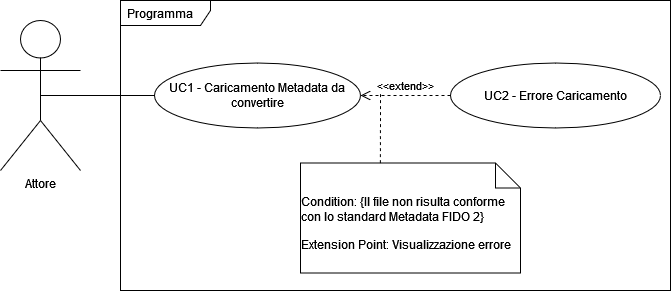
\includegraphics[width=\textwidth]{UC1_UC2.png}
        \caption{Caricamento Metadata}
    \end{figure}

    \begin{itemize}
        \item \textbf{Descrizione:} l'attore vuole convertire un Metdata;
        \item \textbf{Attore primario:} attore;
        \item \textbf{Precondizioni:} l’attore ha a disposizione un Metadata in formato di file;
        \item \textbf{Postcondizioni:} i dati presenti nel Metdata vengono convertiti;
        \item \textbf{Scenario principale:}
        \begin{enumerate}
          \item L'attore avvia l'applicazione;
          \item L'attore sceglie un Metadata da passare all'applicazione;
          \item L'attore carica il Metadata nell'applicazione.
        \end{enumerate}
        \item \textbf{Estensioni:} nel caso in cui il Metadata sia in un formato non valido:
          \begin{enumerate}
            \item Il caricamento non va a buon fine;
            \item Viene visualizzato un errore esplicativo [UC2].
          \end{enumerate}
      \end{itemize}


    \section{UC2 - Errore Caricamento}
    \begin{itemize}
        \item \textbf{Descrizione}: l'attore carica un Metadata mal formattato o che presenta dati non validi, quindi visualizza un messaggio di errore esplicativo;
        \item \textbf{Attore Primario:} attore;
        \item \textbf{Precondizioni:} l’utente carica un Metadata contenente alcuni dati mal formattati o non validi;
        \item \textbf{Postcondizioni:} l'utente visualizza un messaggio di errore e il Metadata non viene caricato;
        \item \textbf{Scenario Principale:}
        \begin{enumerate}
          \item L'utente visualizza un messaggio di errore esplicativo.
        \end{enumerate}
      \end{itemize}

\chapter{Requisiti}
\section{Requisiti Funzionali}

\begin{center}
  \centering
  \begin{longtable}{|L{2cm}|C{5,5cm}|C{3cm}|C{2cm}|}
    \hline
    \rowcolor[HTML]{036400}
    \textcolor[HTML]{FFFFFF}{\textbf{Codice}} & \textcolor[HTML]{FFFFFF}{\textbf{Descrizione}} & \textcolor[HTML]{FFFFFF}{\textbf{Classificazione}} & \textcolor[HTML]{FFFFFF}{\textbf{Fonti}}
    \\ \hline
    \rowcolor[HTML]{EFEFEF}
    RF.1.1 & L'utente deve poter caricare il Metadata & Obbligatorio & UC1 \\ \hline
    \rowcolor[HTML]{C0C0C0}
    RF.1.2 & Visualizzazione messaggio di errore in caso di problemi durante il caricamento del Metadata & Obbligatorio & UC2 \\ \hline
    \rowcolor[HTML]{EFEFEF}
    RF.2.1 & Conversione campo "legalHeader" & Obbligatorio & progetto \\ \hline
    \rowcolor[HTML]{C0C0C0}
    RF.2.2 & Conversione campo "aaid" & Obbligatorio & progetto \\ \hline
    \rowcolor[HTML]{EFEFEF}
    RF.2.3 & Conversione campo "aaguid" & Obbligatorio & progetto \\ \hline
    \rowcolor[HTML]{C0C0C0}
    RF.2.4 & Conversione campo "attestationCertificateKeyIdentifiers" & Obbligatorio & progetto \\ \hline
    \rowcolor[HTML]{EFEFEF}
    RF.2.5 & Conversione campo "description" & Obbligatorio & progetto \\ \hline
    \rowcolor[HTML]{C0C0C0}
    RF.2.6 & Conversione campo "alternativeDescriptions" & Obbligatorio & progetto \\ \hline
    \rowcolor[HTML]{EFEFEF}
    RF.2.7 & Conversione campo "authenticatorVersion" & Obbligatorio & progetto \\ \hline
    \rowcolor[HTML]{C0C0C0}
    RF.2.8 & Conversione campo "protocolFamily" & Obbligatorio & progetto \\ \hline
    \rowcolor[HTML]{EFEFEF}
    RF.2.9 & Conversione campo "upv" & Obbligatorio & progetto \\ \hline
    \rowcolor[HTML]{C0C0C0}
    RF.2.10 & Conversione campo "assertionScheme" & Obbligatorio & progetto \\ \hline
    \rowcolor[HTML]{EFEFEF}
    RF.2.11 & Conversione campo "authenticationAlgorithm" & Obbligatorio & progetto \\ \hline
    \rowcolor[HTML]{C0C0C0}
    RF.2.12 & Conversione campo "authenticationAlgorithms" & Obbligatorio & progetto \\ \hline
    \rowcolor[HTML]{EFEFEF}
    RF.2.13 & Conversione campo "publicKeyAlgAndEncoding" & Obbligatorio & progetto \\ \hline
    \rowcolor[HTML]{C0C0C0}
    RF.2.14 & Conversione campo "publicKeyAlgAndEncodings" & Obbligatorio & progetto \\ \hline
    \rowcolor[HTML]{EFEFEF}
    RF.2.15 & Conversione campo "attestationTypes" & Obbligatorio & progetto \\ \hline
    \rowcolor[HTML]{C0C0C0}
    RF.2.16 & Conversione campo "userVerificationDetails" & Obbligatorio & progetto \\ \hline
    \rowcolor[HTML]{EFEFEF}
    RF.2.17 & Conversione campo "keyProtection" & Obbligatorio & progetto \\ \hline
    \rowcolor[HTML]{C0C0C0}
    RF.2.18 & Conversione campo "isKeyRestricted" & Obbligatorio & progetto \\ \hline
    \rowcolor[HTML]{EFEFEF}
    RF.2.19 & Conversione campo "isFreshUserVerificationRequired" & Obbligatorio & progetto \\ \hline
    \rowcolor[HTML]{C0C0C0}
    RF.2.20 & Conversione campo "matcherProtection" & Obbligatorio & progetto \\ \hline
    \rowcolor[HTML]{EFEFEF}
    RF.2.21 & Conversione campo "cryptoStrength" & Obbligatorio & progetto \\ \hline
    \rowcolor[HTML]{C0C0C0}
    RF.2.22 & Conversione campo "operatingEnv" & Obbligatorio & progetto \\ \hline
    \rowcolor[HTML]{EFEFEF}
    RF.2.23 & Conversione campo "attachmentHint" & Obbligatorio & progetto \\ \hline
    \rowcolor[HTML]{C0C0C0}
    RF.2.24 & Conversione campo "isSecondFactorOnly" & Obbligatorio & progetto \\ \hline
    \rowcolor[HTML]{EFEFEF}
    RF.2.25 & Conversione campo "tcDisplay" & Obbligatorio & progetto \\ \hline
    \rowcolor[HTML]{C0C0C0}
    RF.2.26 & Conversione campo "tcDisplayContentType" & Obbligatorio & progetto \\ \hline
    \rowcolor[HTML]{EFEFEF}
    RF.2.27 & Conversione campo "tcDisplayPNGCharacteristics" & Obbligatorio & progetto \\ \hline
    \rowcolor[HTML]{C0C0C0}
    RF.2.28 & Conversione campo "attestationRootCertificates" & Obbligatorio & progetto \\ \hline
    \rowcolor[HTML]{EFEFEF}
    RF.2.29 & Conversione campo "ecdaaTrustAnchors" & Obbligatorio & progetto \\ \hline
    \rowcolor[HTML]{C0C0C0}
    RF.2.30 & Conversione campo "icon" & Obbligatorio & progetto \\ \hline
    \rowcolor[HTML]{EFEFEF}
    RF.2.31 & Generazione campo "supportedExtensions" & Obbligatorio & progetto \\ \hline
    \rowcolor[HTML]{C0C0C0}
    RF.2.32 & Generazione campo "schema" & Obbligatorio & progetto \\ \hline
    \rowcolor[HTML]{EFEFEF}
    RF.2.33 & "authenticatorGetInfo" & Obbligatorio & progetto \\ \hline
  \end{longtable}
\end{center}


\section{Requisiti di Qualità}

\begin{center}
  \centering
  \begin{longtable}{|L{2cm}|C{5,5cm}|C{3cm}|C{2cm}|}
    \hline
    \rowcolor[HTML]{036400}
    \textcolor[HTML]{FFFFFF}{\textbf{Codice}} & \textcolor[HTML]{FFFFFF}{\textbf{Descrizione}} & \textcolor[HTML]{FFFFFF}{\textbf{Classificazione}} & \textcolor[HTML]{FFFFFF}{\textbf{Fonti}}
    \\ \hline
    \rowcolor[HTML]{EFEFEF}
    RQ.1 & Deve essere fornito il manuale utente & Obbligatorio & progetto \\ \hline
    \rowcolor[HTML]{C0C0C0}
    RQ.2 & Deve essere fornito il manuale sviluppatore & Obbligatorio & progetto \\ \hline
    \rowcolor[HTML]{EFEFEF}
    RQ.3 & Il prodotto deve essere Open-Source & Obbligatorio & progetto \\ \hline
  \end{longtable}
\end{center}

\section{Requisiti di Vincolo}

\begin{center}
  \centering
  \begin{longtable}{|L{2cm}|C{5,5cm}|C{3cm}|C{2cm}|}
    \hline
    \rowcolor[HTML]{036400}
    \textcolor[HTML]{FFFFFF}{\textbf{Codice}} & \textcolor[HTML]{FFFFFF}{\textbf{Descrizione}} & \textcolor[HTML]{FFFFFF}{\textbf{Classificazione}} & \textcolor[HTML]{FFFFFF}{\textbf{Fonti}}
    \\ \hline
    \rowcolor[HTML]{EFEFEF}
    RV.1 & Il prodotto deve essere sviluppato con \textit{Typescript} & Obbligatorio & progetto \\ \hline
    \rowcolor[HTML]{C0C0C0}
    RV.2 & Deve essere sviluppato un Parser per il Metadata FIDO versione 2 & Obbligatorio & progetto \\ \hline
    \rowcolor[HTML]{EFEFEF}
    RV.3 & Deve essere sviluppato un Parser per il Metadata FIDO versione 3 & Obbligatorio & progetto \\ \hline
    \rowcolor[HTML]{C0C0C0}
    RV.4 & Devono essere codificati i test & Obbligatorio & progetto \\ \hline
  \end{longtable}
\end{center}


\section{Riepilogo}

\begin{center}
  \centering
  \begin{longtable}{|c|c|c|c|c|}
    \hline
    \rowcolor[HTML]{036400}
    {\color[HTML]{FFFFFF} \textbf{Tipologia}} & {\color[HTML]{FFFFFF} \textbf{Obbligatorio}} & {\color[HTML]{FFFFFF} \textbf{Obbligatorio}} & {\color[HTML]{FFFFFF} \textbf{Opzionale}}  & {\color[HTML]{FFFFFF} \textbf{Totale}} \\ \hline
    \rowcolor[HTML]{EFEFEF}
    Funzionale & 31 & 3 & 3 & 37 \\ \hline
    \rowcolor[HTML]{C0C0C0}
    Di Qualità & 1 & 1 & 1 & 3 \\ \hline
    \rowcolor[HTML]{EFEFEF}
    Di Vincolo & 3 & 1 & 0 & 4 \\ \hline
    \rowcolor[HTML]{C0C0C0}
    Totale & 35 & 5 & 4 & 44 \\ \hline
    \caption{Tabella del riepilogo totale}
  \end{longtable}
\end{center}